\documentclass[11pt]{report}

% Paquetes y configuraciones adicionales
\usepackage{graphicx}
\usepackage[export]{adjustbox}
\usepackage{caption}
\usepackage{float}
\usepackage{titlesec}
\usepackage{geometry}
\usepackage[hidelinks]{hyperref}
\usepackage{titling}
\usepackage{parskip}
\usepackage[nointegrals]{wasysym}
\usepackage{tikzsymbols}
\usepackage{fancyvrb}
\usepackage{xurl}
\usepackage{subcaption}
\usepackage{amsmath}
\usepackage{multirow}
\usepackage[utf8]{inputenc}
\usepackage{listings}
\usepackage{xcolor}
\usepackage[spanish]{babel}
\usepackage{amsfonts}
\usepackage{amssymb}
\usepackage{booktabs}
\usepackage{array}
\usepackage{verbatim}
\usepackage{url}
\usepackage{pmboxdraw}
\usepackage{dirtree}
\usepackage{longtable}
\usepackage{tabularx}

\usepackage{colortbl}
\usepackage{makecell}
\usepackage{makecell}   % para \thead y saltos de línea en cabecera
\usepackage{pdflscape}  % opcional, si se quiere en apaisado
\usepackage{seqsplit}

\newcommand{\subtitle}[1]{
  \posttitle{
    \par\end{center}
    \begin{center}\large#1\end{center}
    \vskip0.5em}
}

% Configura los márgenes
\geometry{
  left=2cm,
  right=2cm,
  top=3cm,
  bottom=3cm,
}

% Configuración de los títulos de las secciones
\titlespacing{\chapter}{0pt}{\parskip}{\parskip}
\titlespacing{\chapter}{0pt}{\parskip}{\parskip}
\titlespacing{\subsection}{0pt}{\parskip}{\parskip}

% Redefinir el formato de los capítulos y añadir un punto después del número
\makeatletter
\renewcommand{\@makechapterhead}[1]{%
  \vspace*{0\p@}
  {\parindent \z@ \raggedright \normalfont
    \ifnum \c@secnumdepth >\m@ne
        \huge\bfseries \thechapter.\ 
    \fi
    \interlinepenalty\@M
    #1\par\nobreak
    \vspace{10pt}
  }}
\makeatother

% Configura para que cada \chapter no comience en una pagina nueva
\makeatletter
\renewcommand\chapter{\@startsection{chapter}{0}{\z@}%
    {-3.5ex \@plus -1ex \@minus -.2ex}%
    {2.3ex \@plus.2ex}%
    {\normalfont\Large\bfseries}}
\makeatother

% Configurar los colores para el código
\definecolor{codegreen}{rgb}{0,0.6,0}
\definecolor{codegray}{rgb}{0.5,0.5,0.5}
\definecolor{codepurple}{rgb}{0.58,0,0.82}
\definecolor{backcolour}{rgb}{0.95,0.95,0.92}

% Configurar el estilo para el código
\lstdefinestyle{mystyle}{
  backgroundcolor=\color{backcolour},   
  commentstyle=\color{codegreen},
  keywordstyle=\color{magenta},
  numberstyle=\tiny\color{codegray},
  stringstyle=\color{codepurple},
  basicstyle=\ttfamily\footnotesize,
  breakatwhitespace=false,         
  breaklines=true,                 
  captionpos=b,                    
  keepspaces=true,                 
  numbers=left,                    
  numbersep=5pt,                  
  showspaces=false,                
  showstringspaces=false,
  showtabs=false,                  
  tabsize=2
}


\begin{document}

\begin{titlepage}
  \begin{center}
    
\includegraphics[scale=0.5]{img/logo.png}
    \vspace{1cm}

    \vspace{2cm}
    \begin{Huge}
      \textbf{Practica 3: Calidad de la visualización. Checks}
    \end{Huge}

    \vspace{1cm}
    \begin{large}
      \textbf{Visualizaci\'{o}n de Datos}
    \end{large}

    \vspace{4cm}
    \begin{large}
      \textbf{Autor:} Cheuk Kelly Ng Pante (alu0101364544@ull.edu.es)
    \end{large}

    \vspace{1cm}
    \begin{large}
      \textbf{Fecha:} \today
    \end{large}
  \end{center}
\end{titlepage}

\pagestyle{empty}

% Índice
\tableofcontents

% Nueva página
\cleardoublepage

\pagestyle{plain}
\setcounter{page}{1}

\chapter{Utilización del laboratorio de checks}
\section{Análisis de \texttt{test\_checks.py}}
Lo que hace el asset \texttt{islas\_raw} es cargar los datos del CSV y añade intecionalmente una ``fila sucia'' (con el valor ``tenerife'' en minúsculas) para que el check falle. El check \texttt{check\_estandarizacion\_islas} comprueba que no existan errores de formato (mayúsculas/minúsculas). Lo hace comparando la cantidad de categorías únicas originales con las categorías únicas que resultan al normalizar el texto, poniendo la primera letra en mayúscula.

\section{Análisis de \texttt{definitions.py}}
Se incluye el asset \texttt{islas\_raw} importándolo a través del módulo \texttt{test\_checks.py} mediante la función \texttt{load\_assets\_from\_modules}.

En cuanto a los checks que están en manifiesto, se incluye el check \texttt{check\_estandarizacion\_islas} del mismo módulo, cargándolo con la función \texttt{load\_asset\_checks\_from\_modules}.

\section{Lanzamiento y materialización de los assets}
Se lanzó el servidor local mediante el comando:

\begin{verbatim}
dagster dev -f definitions.py
\end{verbatim}

\subsection*{Ejecución del check sin fallos}

Para demostrar el funcionamiento correcto del sistema de checks, se ejecutó también una versión limpia del asset \texttt{islas\_raw} sin la fila sucia. Al materializarla en la interfaz gráfica de Dagster, el check pasó exitosamente (aparece en verde), confirmando que todos los nombres de isla están estandarizados correctamente. Esto valida que el pipeline está preparado para evitar inconsistencias en la visualización y que el sistema de validación funciona como se esperaba.

\begin{figure}[H]
  \centering
  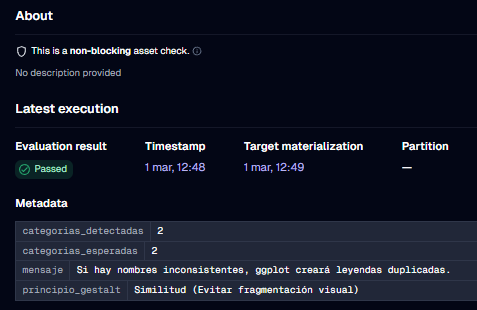
\includegraphics[width=0.7\textwidth]{img/lab_test_checks_passed.png}
  \caption{Interfaz de Dagster mostrando el check pasado correctamente.}
  \label{fig:check_passed}
\end{figure}

\subsection*{Ejecución del check con fallo}

Ahora, para demostrar que el check detecta correctamente los errores, se ejecutó la versión sucia del asset \texttt{islas\_raw} con la fila sucia introducida, demostrando cómo el sistema detecta inconsistencias que generarían leyendas duplicadas en la posterior visualización. En la Figura~\ref{fig:check} se muestra la interfaz de Dagster con el check fallido.

\begin{figure}[H]
  \centering
  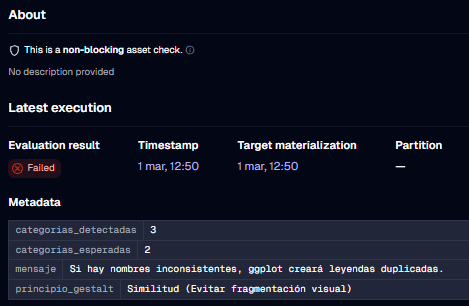
\includegraphics[width=0.7\textwidth]{img/lab_test_checks_failed.png}
  \caption{Interfaz de Dagster mostrando el check fallido.}
  \label{fig:check}
\end{figure}

\chapter{Análisis de la práctica anterior}
El proyecto implementa un pipeline DataOps con Dagster para analizar y visualizar la distribución de la renta en Canarias a partir del dataset oficial del ISTAC, integrando además información territorial y nivel educativo . A través de una arquitectura basada en assets interconectados, se estructura el flujo en tres fases: carga de datos (normalización de columnas, control de nulos y tipado), transformación (filtrado por municipios, agregaciones, cálculo de porcentajes y uniones) y visualización mediante la gramática de gráficos con plotnine (gráficos de barras, barras apiladas y scatter). El diseño sigue principios de calidad visual y perceptiva (orden por magnitud, control de cardinalidad, proporciones coherentes), incorporando checks que garantizan integridad, coherencia semántica y veracidad gráfica, lo que convierte el proyecto en un ejemplo sólido de integración entre ingeniería de datos, análisis estadístico y visualización analítica reproducible.

En la Tabla~\ref{tab:checks_calidad} se resumen los tres checks de calidad implementados en el pipeline, detallando su lógica de programación, su relación con los principios de diseño visual y la información que aportan a los metadatos para facilitar la interpretación de los resultados.

\definecolor{headbg}{RGB}{46, 117, 182}
\definecolor{rawbg}{RGB}{217, 234, 211}
\definecolor{curbg}{RGB}{255, 242, 204}
\definecolor{visbg}{RGB}{207, 226, 255}

\begin{landscape}
\begin{table}[H]
\centering
\caption{Matriz de Calidad -- Checks implementados en el pipeline de rentas}
\label{tab:checks_calidad}
\renewcommand{\arraystretch}{1.6}
\setlength{\tabcolsep}{4pt}
\footnotesize

% Suma total: 2.5+3.5+4.0+3.5+4.0+3.0 = 20.5cm
\begin{tabular}{
  >{\bfseries\raggedright\arraybackslash}p{2.5cm}
  >{\raggedright\arraybackslash}p{3.5cm}
  >{\raggedright\arraybackslash}p{4.0cm}
  >{\ttfamily\raggedright\arraybackslash}p{3.5cm}
  >{\raggedright\arraybackslash}p{4.0cm}
  >{\ttfamily\raggedright\arraybackslash}p{3.0cm}
}

\toprule
\rowcolor{headbg}
\color{white}\textbf{Etapa} &
\color{white}\textbf{Nombre del Check} &
\color{white}\textbf{Descripción Técnica} &
\color{white}\textbf{Cómo programarlo (Lógica)} &
\color{white}\textbf{Relación con el Diseño / Gestalt} &
\color{white}\textbf{Información para Metadata} \\
\midrule

\rowcolor{rawbg}
Carga (Raw) &
{\ttfamily\seqsplit{check\_estandarizacion\_islas}} &
Evita duplicados en la leyenda por inconsistencias de mayúsculas/minúsculas
(ej.\ \texttt{"tenerife"} vs \texttt{"Tenerife"}). &
\seqsplit{df["ISLA"].nunique()==df["ISLA"].str.capitalize().nunique()} &
\textbf{Similitud:} evita que una misma isla se pinte con dos colores distintos
en la leyenda del gráfico. &
\seqsplit{categorias\_detectadas,} \seqsplit{categorias\_esperadas,} mensaje \\

\midrule

\rowcolor{curbg}
Transformación (Curated) &
{\ttfamily\seqsplit{check\_obs\_value\_rango}} &
Detecta valores de porcentaje fuera del rango válido (0\,--\,100) que
indicarían datos corruptos en la carga. &
\seqsplit{(df["OBS\_VALUE"]>=0)\&(df["OBS\_VALUE"]<=100).all()} &
\textbf{Proporcionalidad:} valores fuera de escala comprimen el eje y hacen
que barras correctas parezcan insignificantes. &
\seqsplit{valores\_fuera\_rango,} \seqsplit{min\_valor,} \seqsplit{max\_valor,} mensaje \\

\midrule

\rowcolor{visbg}
Visualización (Asset) &
{\ttfamily\seqsplit{check\_series\_ordenadas}} &
Verifica que los municipios están ordenados ascendentemente por
\texttt{OBS\_VALUE} en el gráfico de barras. &
\seqsplit{valores==sorted(valores)} &
\textbf{Continuidad:} el ojo sigue una escalera suave en lugar de
saltos erráticos, reduciendo el esfuerzo cognitivo. &
\seqsplit{ordenado} (bool), mensaje \\

\bottomrule
\end{tabular}
\end{table}
\end{landscape}

\subsection*{Resultados de la ejecución de los checks}

Tras materializar el pipeline completo en Dagster, los tres checks de calidad
definidos fueron ejecutados automáticamente. A continuación se muestran los
resultados obtenidos en la interfaz web de Dagster.

% ── CHECK 1 ──────────────────────────────────────────────────────────────────
\subsubsection*{Check 1 – Carga: \texttt{check\_estandarizacion\_islas}}

\begin{figure}[H]
    \centering
    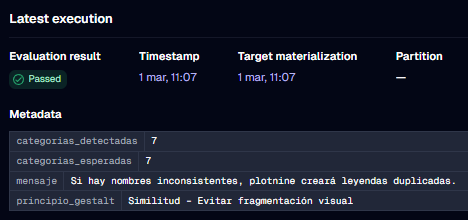
\includegraphics[width=0.75\textwidth]{img/asset_check_1.png}
    \caption{Resultado del check de estandarización de islas sobre \texttt{raw\_codislas}.}
    \label{fig:check1}
\end{figure}

El check ha \textbf{pasado} correctamente. Los metadatos confirman que el número
de categorías detectadas y esperadas coincide (\texttt{categorias\_detectadas = 7},
\texttt{categorias\_esperadas = 7}), lo que indica que todos los nombres de isla
en \texttt{codislas.csv} están escritos de forma consistente. No existe riesgo
de que \texttt{plotnine} genere leyendas duplicadas en los gráficos.

% ── CHECK 2 ──────────────────────────────────────────────────────────────────
\subsubsection*{Check 2 – Transformación: \texttt{check\_obs\_value\_rango}}

\begin{figure}[H]
    \centering
    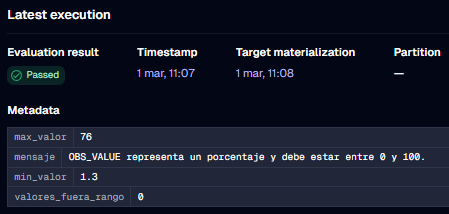
\includegraphics[width=0.75\textwidth]{img/asset_check_2.png}
    \caption{Resultado del check de rango de \texttt{OBS\_VALUE} sobre \texttt{renta\_municipios}.}
    \label{fig:check2}
\end{figure}

El check ha \textbf{pasado} correctamente. Los metadatos muestran que el valor
mínimo es \texttt{1.3} y el máximo \texttt{76}, ambos dentro del rango válido
(0\,--\,100), y que el número de valores fuera de rango es \texttt{0}. Los datos
de porcentaje sobre la renta total son coherentes y no presentan valores corruptos
que pudieran distorsionar la escala del gráfico.

% ── CHECK 3 ──────────────────────────────────────────────────────────────────
\subsubsection*{Check 3 – Visualización: \texttt{check\_series\_ordenadas}}

\begin{figure}[H]
    \centering
    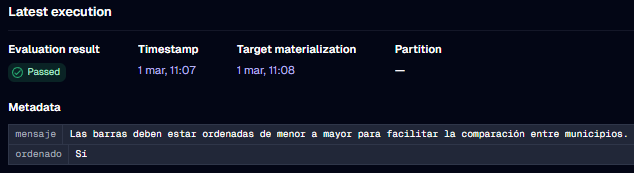
\includegraphics[width=0.75\textwidth]{img/asset_check_3.png}
    \caption{Resultado del check de orden ascendente sobre \texttt{grafico\_renta\_municipios}.}
    \label{fig:check3}
\end{figure}

El check ha \textbf{pasado} correctamente. El metadato \texttt{ordenado = Sí}
confirma que los municipios están ordenados de menor a mayor por su valor de
sueldos y salarios en el gráfico de barras. Esto garantiza que el principio de
\textbf{Continuidad} se cumple: el ojo del lector puede seguir una
escalera visual suave en lugar de encontrar saltos erráticos que aumenten el
esfuerzo cognitivo necesario para interpretar el gráfico.

\newpage

\chapter{Verificación de los checks: casos de fallo}

Para demostrar que los tres checks de calidad detectan correctamente los
errores, se ha creado el fichero \texttt{scripts/casos\_fallo.py}. Este
fichero define tres assets alternativos ---~\texttt{raw\_codislas\_sucio},
\texttt{renta\_municipios\_sucia} y
\texttt{renta\_con\_nombres\_desordenada}~--- cada uno con su propio
\texttt{@asset\_check} asociado. En cada asset se introduce una
\textbf{fila sucia} mediante \texttt{pd.concat} con datos incorrectos
deliberados. El fichero incluye su propio bloque \texttt{Definitions} y
se lanza de forma independiente al pipeline principal, sin modificar ningún
asset de la práctica 2. A continuación se muestran los resultados obtenidos
en la interfaz de Dagster tras materializar cada asset sucio.

% ══════════════════════════════════════════════════════════════════════════════
\subsection*{Caso 1 – Fallo en \texttt{check\_estandarizacion\_islas}}
% ══════════════════════════════════════════════════════════════════════════════
El check ha \textbf{fallado} tal como se esperaba. Los metadatos muestran
que el número de \texttt{categorias\_detectadas} es \textbf{8}, mientras
que el de \texttt{categorias\_esperadas} tras normalizar con
\texttt{str.lower().str.strip()} es \textbf{7}. En el campo
\texttt{islas\_unicas} puede observarse la causa directa: aparecen tanto
\texttt{'Tenerife'} como \texttt{'tenerife'} como categorías distintas,
lo que confirma que la fila sucia ha sido detectada. De no corregirse,
\texttt{plotnine} generaría una entrada duplicada en la leyenda del gráfico,
violando el principio de \textbf{Similitud} de la Gestalt.

\begin{figure}[H]
    \centering
    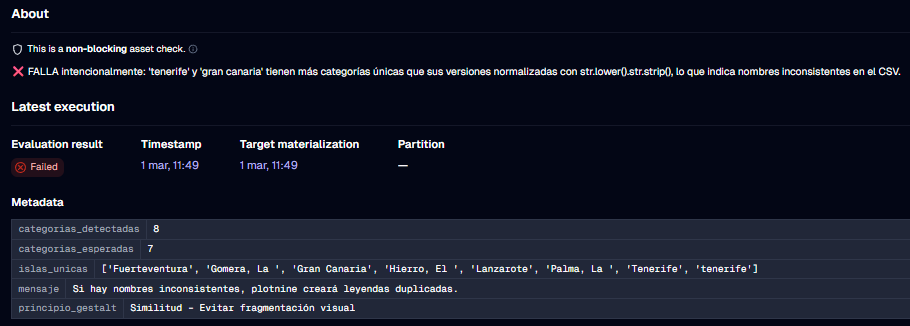
\includegraphics[width=0.85\textwidth]{img/asset_check_1_fail.png}
    \caption{Resultado fallido del check de estandarización de islas sobre
             \texttt{raw\_codislas\_sucio}.}
    \label{fig:check1_fail}
\end{figure}


% ══════════════════════════════════════════════════════════════════════════════
\subsection*{Caso 2 – Fallo en \texttt{check\_obs\_value\_rango}}
% ══════════════════════════════════════════════════════════════════════════════
El check ha \textbf{fallado} tal como se esperaba. Los metadatos confirman
que \texttt{valores\_fuera\_rango} es \textbf{1} y que el \texttt{min\_valor}
registrado es \textbf{-5}, correspondiente a la fila sucia introducida.
El valor máximo sigue siendo \textbf{76}, dentro del rango válido. De no
detectarse, el valor negativo comprimiría el eje Y del gráfico haciendo que
las barras de los municipios correctos parecieran insignificantes, violando
el principio de \textbf{Proporcionalidad}.

\begin{figure}[H]
    \centering
    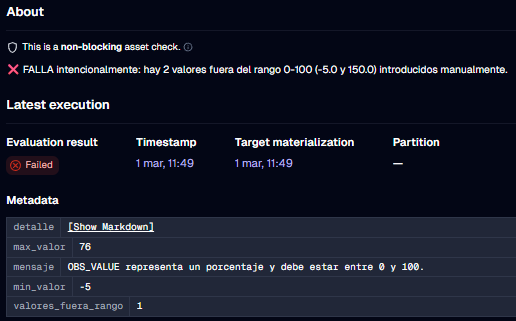
\includegraphics[width=0.75\textwidth]{img/asset_check_2_fail.png}
    \caption{Resultado fallido del check de rango de \texttt{OBS\_VALUE}
             sobre \texttt{renta\_municipios\_sucia}.}
    \label{fig:check2_fail}
\end{figure}


% ══════════════════════════════════════════════════════════════════════════════
\subsection*{Caso 3 – Fallo en \texttt{check\_series\_ordenadas}}
% ══════════════════════════════════════════════════════════════════════════════

El check ha \textbf{fallado} tal como se esperaba. El metadato
\texttt{ordenado} muestra el valor \textbf{No} y en
\texttt{primeros\_valores} puede verse la secuencia
\texttt{[68.3, 57.2, 68.2, 64.8, 58.3]}, que no es ascendente. Esto
confirma que la fila sucia con \texttt{OBS\_VALUE = 999} concatenada al
final ha roto el orden del DataFrame. De no corregirse, el gráfico
presentaría saltos erráticos que aumentarían el esfuerzo cognitivo del
lector, violando el principio de \textbf{Continuidad / Prägnanz} de la
Gestalt.

\begin{figure}[H]
    \centering
    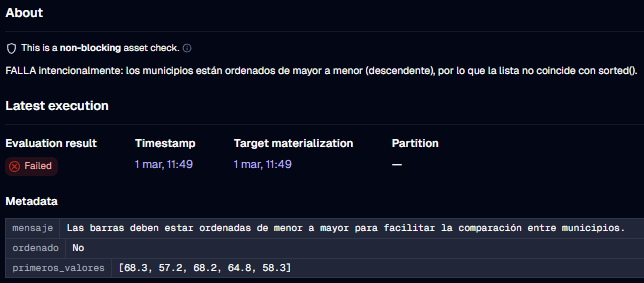
\includegraphics[width=0.85\textwidth]{img/asset_check_3_fail.png}
    \caption{Resultado fallido del check de orden ascendente sobre
             \texttt{grafico\_renta\_municipios\_desordenado}.}
    \label{fig:check3_fail}
\end{figure}

\chapter{Enlace al repositorio de GitHub}
\url{https://github.com/feichay10/Practica_Gramatica_Graficos_DataOps}

\end{document}